\documentclass[a4paper,UTF8,zihao=-4,fontset=fandol]{ctexart}
\usepackage[a4paper,top=25mm,bottom=25mm,left=25mm,right=25mm]{geometry}
\usepackage{graphicx,booktabs,tabularx,array,xcolor,tikz}
\usetikzlibrary{arrows.meta,positioning}
\usepackage{caption}
\usepackage[backend=biber,style=numeric,sorting=none,giveninits=true,doi=false,isbn=false]{biblatex}
\addbibresource{references.bib}
\usepackage[hidelinks,pdfencoding=auto]{hyperref}
\hypersetup{pdftitle={酱菜通——面向江西财经大学的校园学习与生活服务整合应用设计与实现}}
\definecolor{Ink}{HTML}{242A30}
\definecolor{Slate}{HTML}{404B56}
\definecolor{Rule}{HTML}{A2ADB6}
\definecolor{Paper}{HTML}{F2F5F6}
\usepackage{needspace,placeins}
\urlstyle{same}
\ctexset{section={format=\Large\heiti\bfseries\color{Ink},name={第,章},number=\chinese{section},aftername=\quad,beforeskip=16pt,afterskip=9pt},subsection={format=\large\heiti\color{Ink},beforeskip=10pt,afterskip=5pt}}
\setlength{\textfloatsep}{14pt plus 3pt minus 3pt}
\setlength{\intextsep}{12pt plus 3pt minus 3pt}
\captionsetup{font=small,labelfont=bf,skip=6pt,labelsep=quad}
\setlength{\parindent}{2em}
\linespread{1.27}
\setlength{\emergencystretch}{2em}
\renewcommand{\arraystretch}{1.24}
\newcolumntype{Y}{>{\raggedright\arraybackslash}X}
\graphicspath{{figures/}}
\tikzset{
  block/.style={draw=Rule,rounded corners=2pt,fill=Paper,text=Ink,align=center,minimum height=12mm,font=\small,inner sep=4pt},
  link/.style={draw=Slate,semithick,rounded corners=2pt},
  flow/.style={-{Stealth[length=2mm]},semithick,draw=Slate,rounded corners=2pt},
  note/.style={font=\footnotesize,text=Slate,align=center,fill=white,inner sep=2pt}
}
% 封面个人信息。
\newcommand{\studentname}{\rule{65mm}{0.4pt}}
\newcommand{\studentid}{\rule{65mm}{0.4pt}}
\newcommand{\courseinfo}{低代码应用开发}

\begin{document}
\hypersetup{pageanchor=false}
\begin{titlepage}
\centering
\vspace*{30mm}
{\Large\heiti 江西财经大学\par}
\vspace{15mm}
{\LARGE\heiti 个人项目中期实验报告\par}
\vspace{12mm}
{\color{Rule}\rule{0.82\textwidth}{0.5pt}\par}
\vspace{9mm}
{\zihao{1}\heiti 酱菜通\par}
\vspace{5mm}
{\zihao{3}\heiti 面向江西财经大学的校园学习与生活服务整合应用\par}
\vspace{2mm}
{\zihao{3}\heiti 设计与实现\par}
\vspace{19mm}
\begin{tabular}{r@{\hspace{1em}}p{65mm}}
学生姓名 & \studentname \\[5mm]
学\hspace{2em}号 & \studentid \\[5mm]
课\hspace{2em}程 & \courseinfo
\end{tabular}
\vfill
{\small 2026 年 11 月\par}
\end{titlepage}

\pagenumbering{arabic}
\linespread{1.25}\selectfont
\hypersetup{pageanchor=true}
\section{项目背景与需求分析}

\subsection{项目背景}
选题来自学生在同一时段内处理多类校园事务的经历。以准备次日上课为例，学生先查教务课表确认节次和教室，再到学习通检查作业、考试或活动，最后把平台之外的个人事项另记一份。每项操作都已有服务承接，真正重复的是寻找入口、判断消息归属和确认上次查询是否仍然有效。校园饮水和洗浴又各自依赖不同账户。分散带来的困难有两层。学生先要判断该从哪个入口查起，随后还要判断看到的是平台刚返回的结果、上次保存的内容，还是一次查询失败后的空白。以跨周调课为例，知道课程名称并不足以确定走课路线，还需要核对周次与地点。以提交作业为例，看到课堂活动的标题也不能直接判断任务是否仍待处理。酱菜通由此以校园助手为主题，将分散的服务入口集中起来，并清楚呈现查询结果及其状态。

\subsection{开发动机与目标}
本项目将学生每天重复打开的入口收进一个应用。课表适合作为启动后的首屏，进入首页即读本机最近成功数据，随后按条件同步。学习页以任务和教学班为组织单位，提供类型、状态及课程分组，便于在课前判断哪些工作仍待处理。待办页负责个人自行添加的事项，网络不可用时仍可编辑和恢复。生活页集中饮水与洗浴入口，并以服务实际接入状态决定可用操作。我将整合范围限定在共同的入口和操作习惯。课表沿着学期、周次和星期查看，学习页按教学班和任务状态收拢信息，个人待办独立编辑，生活数据继续以各服务的账号和回执为准。

\subsection{目标用户与主要需求}
本项目主要面向江西财经大学在校学生，围绕课程查询、学习任务、个人待办及校园生活服务等日常需求展开设计。走课场景关注课程时间与地点，要求课表在网络波动时仍可查阅。学习管理场景关注是否待交、何时截止，以及哪个教学班发布了任务，过期记录仍应可追溯。个人待办要求保存简单、完成状态可反转。余额和账单等生活数据则需要从本人会话读取，账号失效后应有明确重连路径。这些场景分别对应三项设计判断。课表是走课时需要立即查到的信息，因此启动优先回读，保留更新状态；学习通和待办都可以用状态筛选，但前者采用平台任务状态，后者的完成标记由本人编辑。余额及交易依赖外部会话，因此用户可以集中查看连接状态，并在准备好时主动重连。

\subsection{功能范围}
项目聚焦校园信息查询、任务组织和本机操作。学校成绩和考试安排以校方查询结果为准，学习通开放任务跳转，独立待办由本机保存。慧生活798提供独立的设备和积分流程，实际出水或积分扣减等动作须由用户明确操作。住理生活的原生接入仍处于部分实现，服务页显示设备接口状态并提供官方入口。项目以现有校方和第三方服务提供动态数据，应用直接在本机完成整理和缓存。

\section{参考项目与总体设计}
\subsection{参考项目}
酱菜通面向江西财经大学学生，主要任务是在一个客户端内组织课表、学习任务、个人待办与生活查询。页面和数据整理采用本地 WebView 与 JavaScript，登录会话、受控网络请求及系统能力由 Java 原生层处理。已有组件与目标校园的实际条件决定了各模块的实现范围。江财校历和课表以校方数据为准，待办可在离线环境完整使用，各外部服务仍分别授权。

航院通为移动端架构提供参考。酱菜通沿用其中的 WebView 与 Java 桥接方式，复用了学习通的部分查询、解析、扫描与排序代码\cite{hangyuan}。慧生活798以 life-798 为主要技术参考，用于理解设备账号与积分账号的分工、验证码流程与会话管理，并核对余额、设备、用水控制、账单和积分处理\cite{life798}。排查真实登录问题时，另以已验证可登录的客户端核对请求及会话行为，具体过程见第四章。

\subsection{酱菜通的设计与实现}
江财教务的学期选项、周次表达和成绩报表需要依据实际校方页面处理。酱菜通在同一课程模型中连接校历、课程时段与缓存，并集中提供教务会话的授权及重连入口。学习任务使用教学班组织，活跃度规则另外判断课程是否在默认列表中显示，避免把历史课程和重要任务一并过滤。个人待办用于记录平台之外的日常事务，数据写入本机后可以独立于各服务的登录状态使用。生活页与账号中心分别承接业务操作和授权反馈，住理生活按当前接入状态提供官方服务入口。表\ref{tab:compare}列出这些设计及相关参考。

\begin{table}[htbp]
\centering\caption{酱菜通主要业务及技术参考}\label{tab:compare}
\small
\begin{tabularx}{\linewidth}{@{}>{\raggedright\arraybackslash}p{23mm}YY@{}}
\toprule
业务领域 & 酱菜通设计与实现 & 借鉴的技术思路 \\
\midrule
移动端架构 & 区分应用主界面、校方认证和本机存储的职责 & WebView 与 Java 桥接的端侧组织 \\
江财教务 & 校方课表读取、校历映射、有效成绩与考试报表查询 & 校园服务的模块分组 \\
学习任务 & 同轮处理教学班分项任务与隐藏课程复查，按账号保存可见偏好 & 分项读取、解析、扫描与任务排序 \\
校园生活 & 分别管理设备和积分账号，提供用水查询，并依接入状态展示洗浴入口 & life-798 的双账号分工、验证码流程和业务请求 \\
待办与设置 & 本地保存待办，集中处理账号连接与重连，统一页面层级 & 服务账号和业务页面的入口组织 \\
\bottomrule
\end{tabularx}
\end{table}

\subsection{系统总体架构}
图\ref{fig:arch}展示从页面操作到服务返回的两条数据路径。主界面由 Android 承载本地 HTML、CSS 与 JavaScript。受信的应用页面把请求参数交给 Java 桥接，原生层管理请求范围和对应会话，再将结果送回页面的回调。学习通和798沿用这一路径，JavaScript 负责把响应整理成页面可使用的条目，再按业务状态刷新列表。需在网页内完成的校方认证及页面读取走独立 WebView，院校数据返回主界面前再核验账号、学期和结构。本项目把主界面和外部网页分开，避免面向应用资产的原生能力被注入到认证网页中。

本机保存内容按用途安排。课表及学习结果首先服务于回读，课表按账号与学期隔离，学习缓存按账号隔离。待办和主题偏好用本机 WebView 存储。需要保存的原生凭据由应用私有存储承载，使用 Android Keystore 中的密钥进行加密，代码采用 AES/GCM。凭据留在原生层管理，页面只需获得完成查询所需的返回数据和连接状态。将业务缓存、用户自己录入的待办和会话分别保存，也使普通网页缓存清理可以保留账号及待办。

\begin{figure}[htbp]
\centering\begin{tikzpicture}
\node[block,text width=91mm] (web) at (0,0) {应用主界面 WebView\\操作、业务模型与结果展示};
\node[block,text width=43mm] (bridge) at (-4.05,-1.8) {Java 原生桥接\\受控请求与结果回调};
\node[block,text width=43mm] (portal) at (4.05,-1.8) {独立教务 WebView\\主动认证与后台页面读取};
\node[block,text width=42mm] (store) at (0,-3.6) {本机存储\\缓存、待办和原生凭据};
\node[block,text width=35mm] (vendor) at (-5.35,-3.6) {学习通／798};
\node[block,text width=35mm] (school) at (5.35,-3.6) {江财教务门户};
\draw[flow,<->] (web.south -| bridge.north) -- (bridge.north);
\draw[flow,<->] (web.south -| portal.north) -- (portal.north);
\draw[flow,<->] (web.south) -- node[note,right,pos=.63] {业务数据} (store.north);
\draw[flow,<->] (bridge.south) -- ++(0,-3mm) -| (vendor.north);
\draw[flow,<->] (portal.south) -- ++(0,-3mm) -| (school.north);
\draw[flow,<->] (bridge.east) -| node[note,above,pos=.27] {凭据} ([xshift=-10mm]store.north);
\end{tikzpicture}

\caption{本地页面、原生桥接和外部服务的数据流}\label{fig:arch}
\end{figure}

\subsection{功能模块组织}
功能结构见图\ref{fig:modules}。底栏按任务场景安排，账号管理集中在“我的”。教务、学习通、798设备账号、798积分账号和住理生活在这里显示各自的连接状态。业务页负责查询和查看结果，设置页承接用户明确发起的绑定或重连。这个划分在课表失效时尤其重要，课表仍可保留原有内容，用户自行决定何时重新认证。

\begin{figure}[htbp]
\centering\begin{tikzpicture}
\node[block,text width=46mm] (app) at (0,0) {酱菜通};
\foreach \x/\name/\content in {
  -5.86/a/{教务\\课表\\成绩与考试},
  -2.93/b/{学习\\任务筛选\\课程活跃度},
  0/c/{待办\\编辑与完成\\离线保存},
  2.93/d/{生活\\798 饮水\\住理生活},
  5.86/e/{我的\\账号管理\\外观与缓存}
}{
  \node[block,text width=24mm,minimum height=22mm,font=\footnotesize] (\name) at (\x,-2.1) {\content};
  \draw[flow] (app.south) -- (0,-1.0) -| (\name.north);
}
\end{tikzpicture}

\caption{五个业务模块及其功能分组}\label{fig:modules}
\end{figure}

\section{核心功能设计与实现}

\subsection{教务信息管理}
江财教务采用真实校方会话。Android 9 及以上在独立环境中打开官方门户，由用户完成校方登录。应用将校方登录和普通同步拆为两条入口。首次绑定或重连时，账号中心打开交互认证窗口，读取过程先核验本人课表和对应学期，再发布绑定状态。之后的常规查询由独立后台服务复用已有会话，后台读取不会把认证界面推到前台。读取课表时解析校方个人课表网格，转换为包含课程名称、星期、节次范围、周次和地点的统一课程时段。每条记录按上课时段解释，不将同名课程的不同安排合并。周次条件决定条目是否落在选中教学周，起止节次决定其当天的时间范围，校历再把教学周及星期映射为实际日期。这让周视图与日视图可以使用同一批条目。经核验的学期和不支持的结构分别处理，解析失败时保留原缓存。

同步控制依次判断绑定、缓存状态和本次是否需要请求，流程如图\ref{fig:jufe}所示。一般刷新使用六小时新鲜度，重复请求有三十秒限制；手动刷新可跳过新鲜度判断，仍受重复请求限制。页面优先读取当前账号当前学期缓存，新的数据通过校验才替换。本地条目按账号和学期读取。网络错误或解析失败时继续显示已有可用记录，发现账号不匹配则暂停旧缓存的展示。调度区分等待核验与已确认失效，后者持久化为待重连状态，页面恢复也不会重新触发校方认证。

成绩有效记录来自校方相应查询选项。“入学以来”用于整理有记录的学期目录，选择某学期后复核返回报表的学期标识，结果暂存在内存中。成绩、学分和绩点使用校方字段。考试安排沿用校方开放的学期和批次，不通过改写参数扩大范围。当前证据支持空报表的识别，尚缺非空考试报表的实读复核。

\begin{figure}[htbp]
\centering\begin{tikzpicture}
\node[block,text width=37mm] (open) at (-5.2,0) {进入教务或手动刷新};
\node[block,text width=40mm] (cache) at (0,0) {回读同账号、同学期\\最近可用课表};
\node[block,text width=39mm] (decide) at (5.2,0) {检查会话与刷新条件};
\node[block,text width=39mm] (read) at (5.2,-2.0) {后台读取个人课表};
\node[block,text width=40mm] (check) at (0,-2.0) {核验账号、学期与结构};
\node[block,text width=37mm] (save) at (-5.2,-2.0) {保存结果并更新页面};
\node[block,text width=62mm] (keep) at (0,-4.15) {保留可用课程与同步状态\\确认会话失效时提示主动重连};
\draw[flow] (open) -- (cache);
\draw[flow] (cache) -- (decide);
\draw[flow] (decide) -- node[note,right] {允许刷新} (read);
\draw[flow] (read) -- (check);
\draw[flow] (check) -- node[note,above] {通过} (save);
\draw[flow] (check) -- node[note,left] {读取或校验失败} (keep);
\draw[flow] (decide.east) -- ++(3.5mm,0) |- node[note,pos=.84,above] {无需刷新或会话失效} (keep.east);
\end{tikzpicture}

\caption{课表缓存回读与静默同步流程}\label{fig:jufe}
\end{figure}

\subsection{学习通任务聚合}
同名课程可能分属不同教学班，扫描和缓存以课程与教学班标识共同区分。一次扫描先得到教学班列表，再对作业、考试与活动分项查询，记录各自是否完整。聚合时把活动中重复出现且已在作业分项得到的记录去重，再挂接所属教学班及展示所需字段。归并后的任务保留类型、状态、发布或截止信息及可用链接。列表按紧急程度或课程分组，也可按类型及完成状态过滤。例如待批阅作业保留在已完成一侧，缺少可靠绝对截止时间时保留平台提供的可用表达。分页不完整或分项查询失败时，已有有效分项可继续显示。

课程活跃度处理在扫描结果之后，如图\ref{fig:study}所示。设计时选择通知和作业作为观察依据，稳定标识用于区分新记录与旧记录重复出现。确认无更新需要同时具备可用的通知和作业证据。可靠的发布时间用于计算最近活动，稳定的新标识可以补充缺少发布时间的完整记录。首次确认完整但为空的列表从首次可靠观察起算。来源未读全时保留旧状态，避免因查询失败错误隐藏整门教学班。自动隐藏仅影响默认展示。隐藏或活跃度未知的教学班到达十二小时检查间隔后，由同一扫描流程复核。可靠的新作业或通知会撤销自动隐藏，手动隐藏仍由用户解除。手动隐藏和始终显示偏好随账号缓存保存，继续由用户管理。

\begin{figure}[htbp]
\centering\begin{tikzpicture}
\node[block,text width=37mm] (scan) at (-5.2,0) {有效会话\\扫描教学班与分项任务};
\node[block,text width=40mm] (merge) at (0,0) {解析、去重、归并\\失败分项保留旧结果};
\node[block,text width=39mm] (observe) at (5.2,0) {检查作业和通知\\时间、标识及完整性};
\node[block,text width=37mm] (view) at (-5.2,-2.1) {按类型、状态或课程\\筛选并展示可见任务};
\node[block,text width=40mm] (cache) at (0,-2.1) {按账号保存任务及\\活动证据和可见状态};
\node[block,text width=39mm] (state) at (5.2,-2.1) {超期隐藏，有新内容恢复\\证据不足时保留原状态};
\draw[flow] (scan) -- (merge);
\draw[flow] (merge) -- (observe);
\draw[flow] (observe) -- (state);
\draw[flow] (state) -- (cache);
\draw[flow] (cache) -- (view);
\draw[flow] (cache.south) -- (0,-3.45) -- node[note,midway,below] {到期后隐藏项也参与复查} (-7.4,-3.45) |- (scan.west);
\end{tikzpicture}

\caption{学习通任务聚合与课程活跃度的处理顺序}\label{fig:study}
\end{figure}

\subsection{本地待办管理}
待办用本机唯一标识定位记录，保存标题、备注、截止日期、完成标记和创建、更新及完成时间。用户先输入标题建立未完成记录，需要时打开详情补录备注及截止日期。新增和编辑共用字段校验，只有整份记录写入成功才更新界面。勾选完成会写入完成时间，取消勾选则清除这一时间。删除要求二次确认，重启后从应用私有 WebView 存储恢复。列表中的未完成、已完成和全部是同一数据集的筛选结果。待办独立于教务、学习和生活的登录会话，失去外部网络连接时仍可完成新增、编辑和筛选。这为现场演示提供了一条不依赖第三方服务的完整流程。

\subsection{校园生活服务}
酱菜通参照 life-798 的双账号分工和验证码流程，为798设备账号和积分账号分别管理登录通道与会话。设备通道由本人完成验证码登录。账户会话建立后，余额、收藏设备和消费账单分别发起查询并显示平台返回结果。0.8.9 的记录覆盖了这三项数据，并在冷启动后确认会话恢复及再次读取。设备开始与结束需要用户明确触发，连接结果不确定时优先核查已有状态。积分通道具备余额、钱包、任务、签到及兑换流程的代码，实际积分登录、兑换和启停交易仍有单独的验收条件。用户未在阶段验证中发起这些操作。饮水模块使用 jsQR 解析设备二维码，其 Apache 2.0 许可文件随项目保留。

住理生活在生活页单独显示麦庐园项目。官方 App 可按楼栋、楼层和房间选择设备。酱菜通已实现列表与连接状态的界面和逻辑，缺少获准的真实原生数据源时展示当前状态，并提供官方 App 入口。原生洗浴连接、余额、消费记录和设备控制均未在真实环境中验证。

\subsection{统一账号管理}
整合前，用户可能从多个业务页分别寻找登录按钮，一次会话失效也容易在不同页面收到重复提示。统一后的账号中心集中处理绑定、重连与退出状态，继续由各平台自行认证。教务在校方门户完成授权，学习通复用其账号会话，798设备和积分会话可分别管理，住理生活维持独立的服务状态。对学习通和课表，账号校验也参与缓存回读和更新过程，降低切换账号后复用旧数据的可能。业务页保留查询入口，进入重连时转到账号中心的相应服务。这样课表即便保留了旧缓存，也能清楚地提示需要重新认证，用户可以继续读课表并择时处理会话。

\section{项目开发与迭代优化}

\subsection{初始开发与实际安排}
项目初期先搭建可运行的客户端，用示例课表与本地数据检验页面组织和课程模型，再接入江财教务、学习通与校园生活服务。校方课表结构需要逐步验证，饮水登录也经过多次排查。开发因此调整了顺序，优先解决教务登录循环和缓存显示，并先在生活模块验证真实账户查询。随后完善独立待办和课程活跃度管理，并集中整理账号入口及各页交互。图\ref{fig:timeline}概括了主要阶段及其成果。

\begin{figure}[htbp]
\centering\begin{tikzpicture}
\node[block,text width=29mm,minimum height=21mm] (a) at (-6,0) {\textbf{初步设计}\\客户端与课表模型};
\node[block,text width=29mm,minimum height=21mm] (b) at (-2,0) {\textbf{教务接入}\\课表同步\\会话处理完善};
\node[block,text width=29mm,minimum height=21mm] (c) at (2,0) {\textbf{核心业务完善}\\待办、任务管理\\饮水服务查询};
\node[block,text width=29mm,minimum height=21mm] (d) at (6,0) {\textbf{使用流程整合}\\集中管理账号\\统一界面设计};
\foreach \first/\last in {a/b,b/c,c/d}{\draw[flow] (\first) -- (\last);}
\end{tikzpicture}

\caption{项目主要开发与迭代阶段}\label{fig:timeline}
\end{figure}

\subsection{教务接入与启动登录循环}
初期的模拟适配器和本地导入可以验证课程模型及离线展示，但更新课表仍需用户准备材料。实际检查发现，校方登录首页不足以定位课表，个人课表则包含星期、周次、节次及地点等可解析信息。酱菜通在用户认证后读取个人课表，以独立的校历映射处理校方学期选项，再将读取、校验与缓存更新串成自动同步流程。261 和 252 两个学期均取得真实课表，原有课程模型也继续用于展示同步结果。

接入后，模拟器上的冷启动曾反复弹出教务认证窗口。检查发现，会话已过期与启动后尚待核验共用一条路径，认证窗口关闭后，主界面恢复又满足原来的触发条件。为此，酱菜通将主动授权和静默读取分开，使用独立服务核验会话，并记下已确认的失效状态。实验中，用户主动重连后手动触发后台读取，更新时间随之推进，主界面保持可用。离线或会话失效时，应用仍显示原缓存。这次实验验证了后台读取路径，未等待六小时周期自行触发。

成绩查询也经历了从观察到调整的过程。校方默认选项曾返回空报表，我在校方页面核对了“有效成绩”的查询步骤。酱菜通随后从“入学以来”的报表识别有记录的学期，再按学期核验成绩。实验成功切换 252、251、242、241 四个学期，切回后确认缓存可用。这说明成绩页需要按校方可查结果组织学期，独立于课表能够展示的学期范围。

\subsection{学习通扫描及课程管理}
早期页面已能读取课程任务，但历史教学班与当前课程共同占用列表。按创建时间直接筛除旧教学班，会遗漏在旧课程中重新发布的内容。酱菜通以作业和通知的变化判断活跃度，分别保存可见状态和最近检查信息。统一后的扫描在同一轮读取分项任务，并检查到期的隐藏课程，课程列表和任务筛选共享查询结果。

一次真实扫描共处理 63 个教学班，其中 55 个完成全部分项读取，另有 8 个教学班的部分信息未完整返回。这个结果说明完整性需要按分项判断，成功读取的结果可以继续使用。实测也确认，隐藏课程仍可进入作业和活动复查。三十天阈值、新内容恢复以及旧标识重新出现时的处理通过合成输入检验

\subsection{798 协议适配和真实登录}
酱菜通早期发送短信验证码时取得业务码 0，登录请求却返回 $-1$。收到短信只确认了申请环节。酱菜通对照 life-798 的图形码标识、短信和登录请求、双账号通道与会话管理，定位了可逐项核查的协议边界。此后调整了图形码状态、会话保持及签名配置，并核对了旧版调用链，模拟器和真机仍出现登录失败。已有记录无法把拒绝归因于单一字段。

为进一步缩小排查范围，核对可用客户端的请求行为，并逐项核查请求头、序列化和原生会话行为，然后构建新的请求和页面处理代码，接入本机网络桥接与独立会话存储。完成短信验证后，登录返回业务码 0，随后读取了余额、收藏设备和消费账单，重启后仍可查询。

\subsection{页面布局和操作流程}
账号中心统一了授权入口后，课表页下方仍有重复登录卡和旧导入入口，“我的”也保留了一张独立介绍卡。项目移除这些容器，并继续允许从账号中心重连和回读已保存的课表。界面改进随后调整配色、标题层级、数据列表和弹层布局，让不同模块使用一致的视觉规则。图\ref{fig:beforeafter}展示同一测试账户、同一示例课表在 360 dp 视口下的效果。两张画面按相同范围裁切。修改前后均可选择学期和周次、切换周视图与日视图并刷新课表。

\begin{figure}[!htb]
\centering
\begin{tabular}{@{}c@{\hspace{5mm}}c@{}}
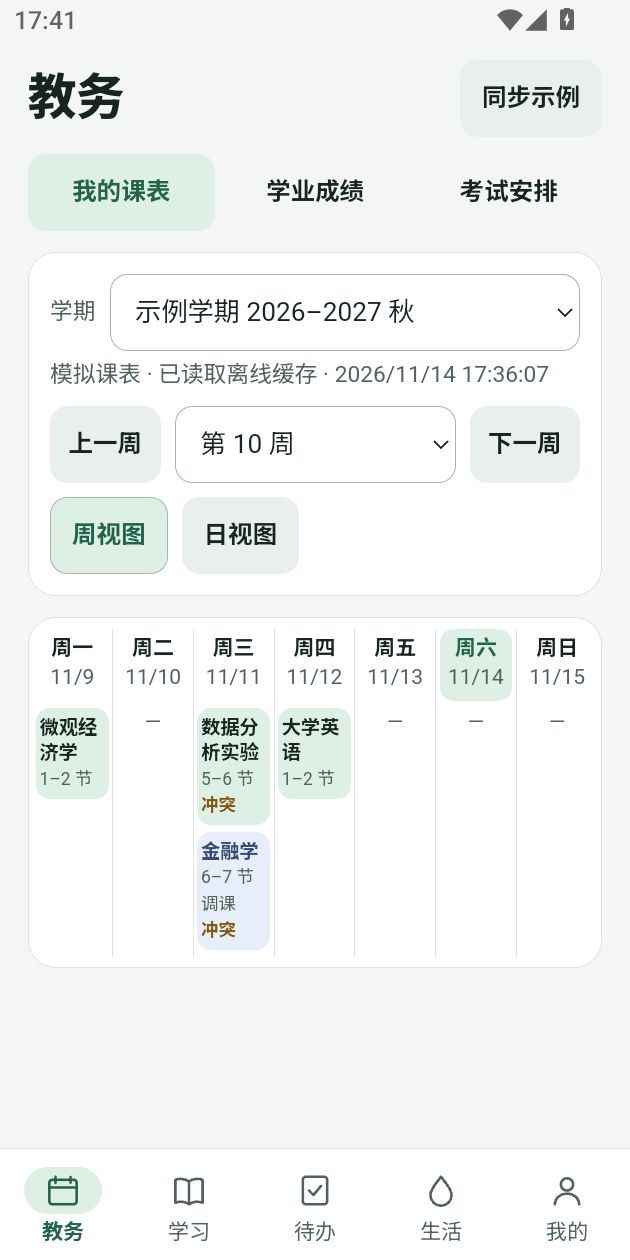
\includegraphics[width=.41\linewidth,trim=0bp 234bp 0bp 36bp,clip]{before-schedule.png} &
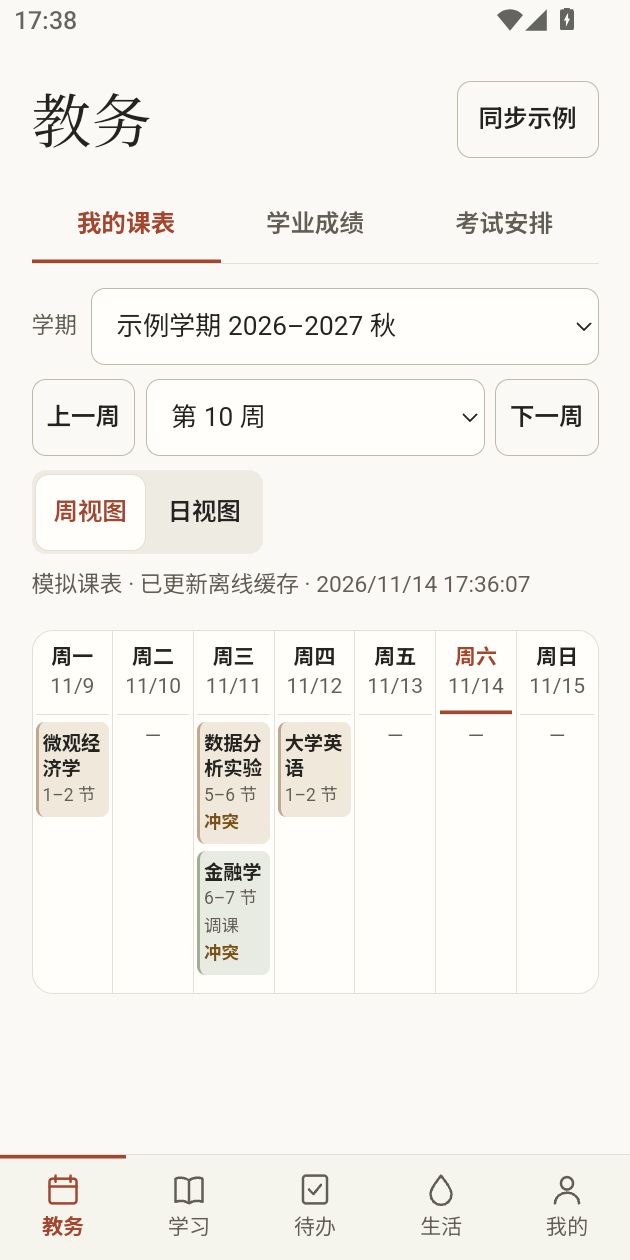
\includegraphics[width=.41\linewidth,trim=0bp 234bp 0bp 36bp,clip]{after-schedule.png} \\
\small 0.9.2 & \small 0.9.3 \\
\end{tabular}
\caption{同尺寸模拟器中的教务课表前后对比}\label{fig:beforeafter}
\end{figure}

\subsection{迭代效果分析}
表\ref{tab:changes}将发现的问题、改进措施和观察到的结果并列。由此可以看出，缓存显示、任务分项完整性与真实账户查询分别需要通过不同的操作验证。

\begin{table}[!htb]
\centering\small
\caption{代表性迭代的问题、措施及实际效果}\label{tab:changes}
\begin{tabularx}{\linewidth}{@{}>{\raggedright\arraybackslash}p{33mm}YY@{}}
\toprule
问题与证据 & 修改及其依据 & 验证结果 \\
\midrule
课表更新依赖手工准备材料 & 已授权页面能读到个人课表，遂以校方网格及校历驱动原有模型 & 两个学期读取成功，自动同步可替换同账号同学期旧结果 \\
会话失效后多次弹出认证 & Activity 恢复反复触发旧逻辑，分离交互认证与静默读取 & 主动重连后后台同步成功，离线和失效时保留课表 \\
历史课程影响当前任务查找 & 采用通知和作业判定活跃度，隐藏项仍纳入原扫描调度 & 实际扫描保留已读分项，隐藏项可继续复查，恢复规则通过合成测试 \\
798 短信成功后登录被拒 & 参考 life-798 分析流程，借可登录客户端确认请求与会话差异 & 本人登录后读取余额、设备与账单，重启后可以再次查询 \\
\bottomrule
\end{tabularx}
\end{table}

\FloatBarrier
\section{项目成果与功能验证}

\subsection{开发与实验环境}
项目在 Windows 上开发，采用 HTML、CSS 和 JavaScript 编写应用内页面，由 Android WebView 加载。页面通过 Java 原生桥接访问外部服务，原生层负责会话管理，返回的数据由页面整理和展示。应用的安装、启动和页面交互在 MuMu 的 Android 15 环境中检验。实验分为实际账户查询、本机操作和合成输入检查。实际账户查询用于核对服务能否返回可用结果，本机操作用于检查界面和数据保存，合成输入用于验证阈值、筛选及异常处理等可控条件。图示采用当前版本的运行画面，保留了对早期业务实验结果的独立说明。

\subsection{主要界面与运行成果}
上一章图\ref{fig:beforeafter}已展示新版课表操作区。图\ref{fig:run-main}进一步展示学习入口与待办操作区。待办界面可见实际输入区、状态筛选和已有测试事项，学习截图使用未连接的测试账户。图\ref{fig:run-other}把生活入口与统一账号列表相邻呈现。饮水页提供登录入口，账号列表呈现五项服务各自的状态。“我的”仍设有外观与缓存管理。生活页与账号中心同样使用未授权的测试账户，展示的是接入入口与连接状态。

\begin{figure}[!htb]
\centering
\begin{tabular}[t]{@{}c@{\hspace{5mm}}c@{}}
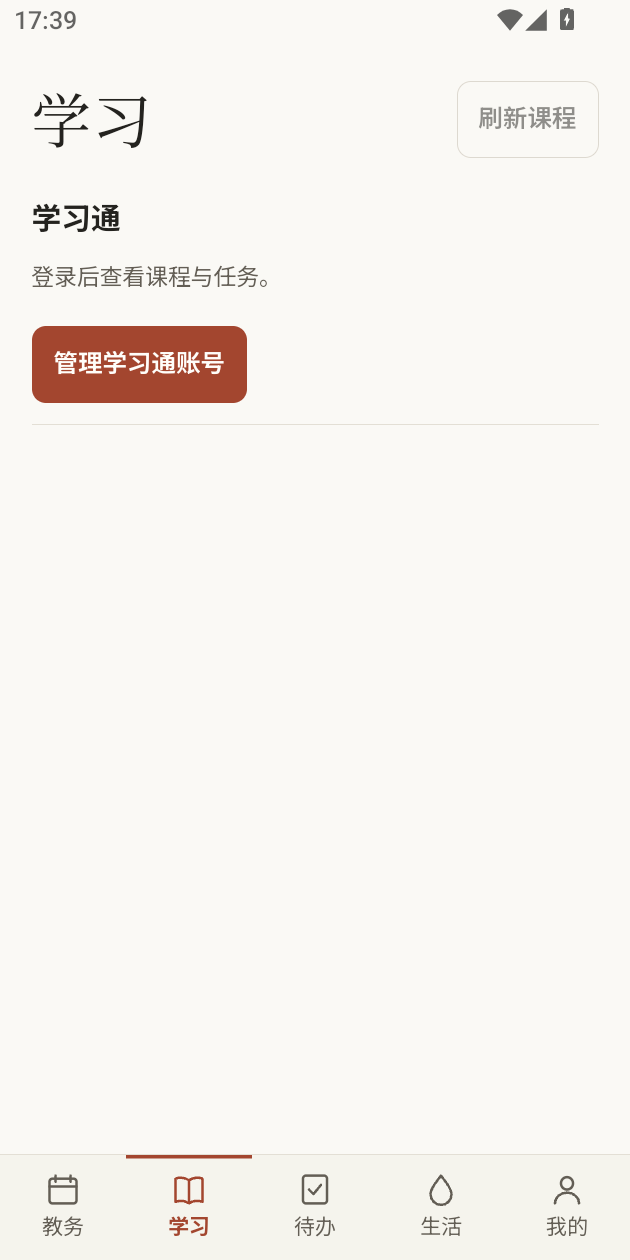
\includegraphics[width=.46\linewidth,trim=0bp 585bp 0bp 34bp,clip]{after-study.png} &
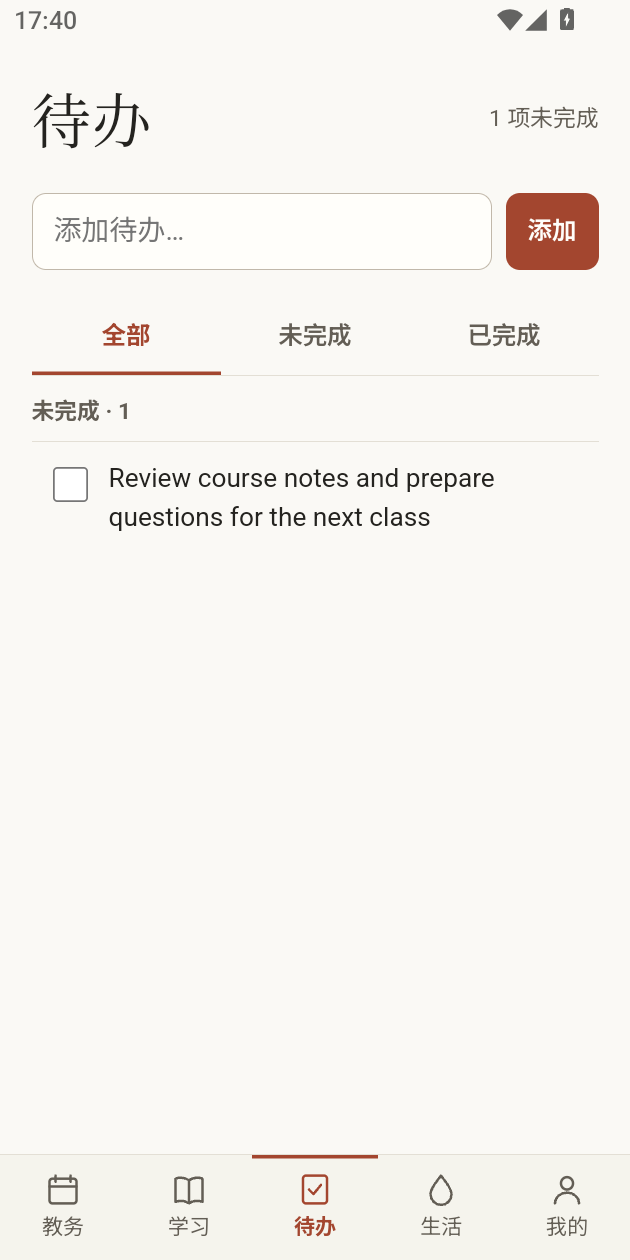
\includegraphics[width=.46\linewidth,trim=0bp 585bp 0bp 34bp,clip]{after-todo.png} \\
\small （a）学习入口 & \small （b）本地待办
\end{tabular}
\caption{学习入口与本地待办的实际操作区域}\label{fig:run-main}
\end{figure}

\begin{figure}[!htb]
\centering
\begin{tabular}[t]{@{}c@{\hspace{5mm}}c@{}}
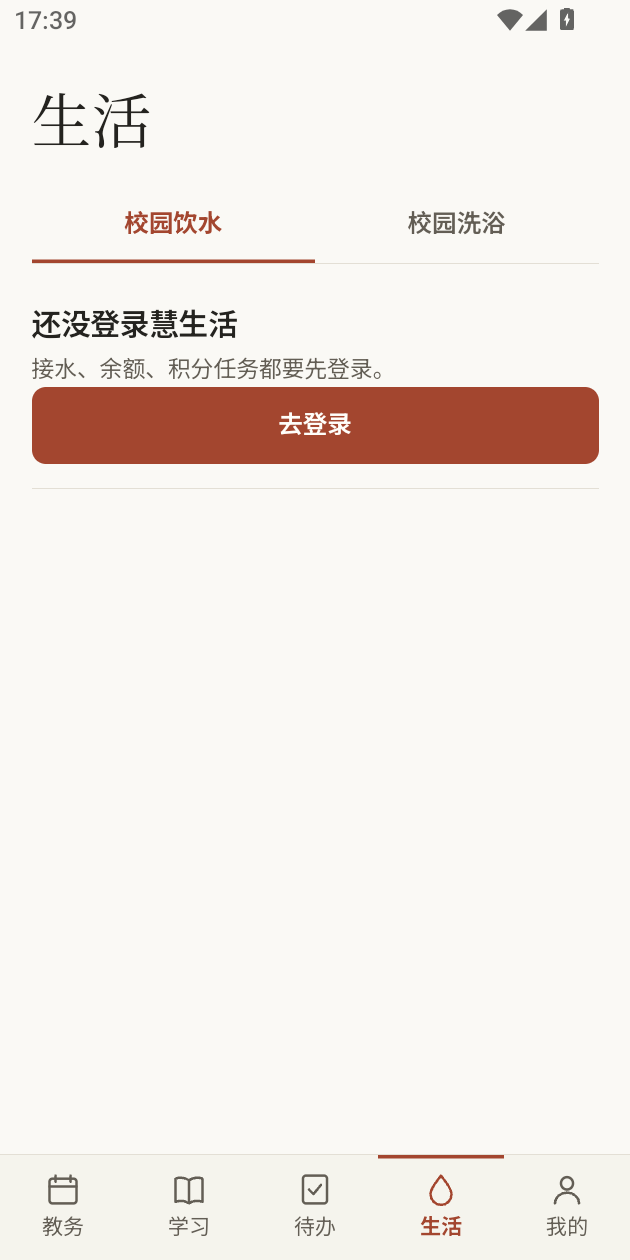
\includegraphics[width=.46\linewidth,trim=0bp 466bp 0bp 34bp,clip]{after-life.png} &
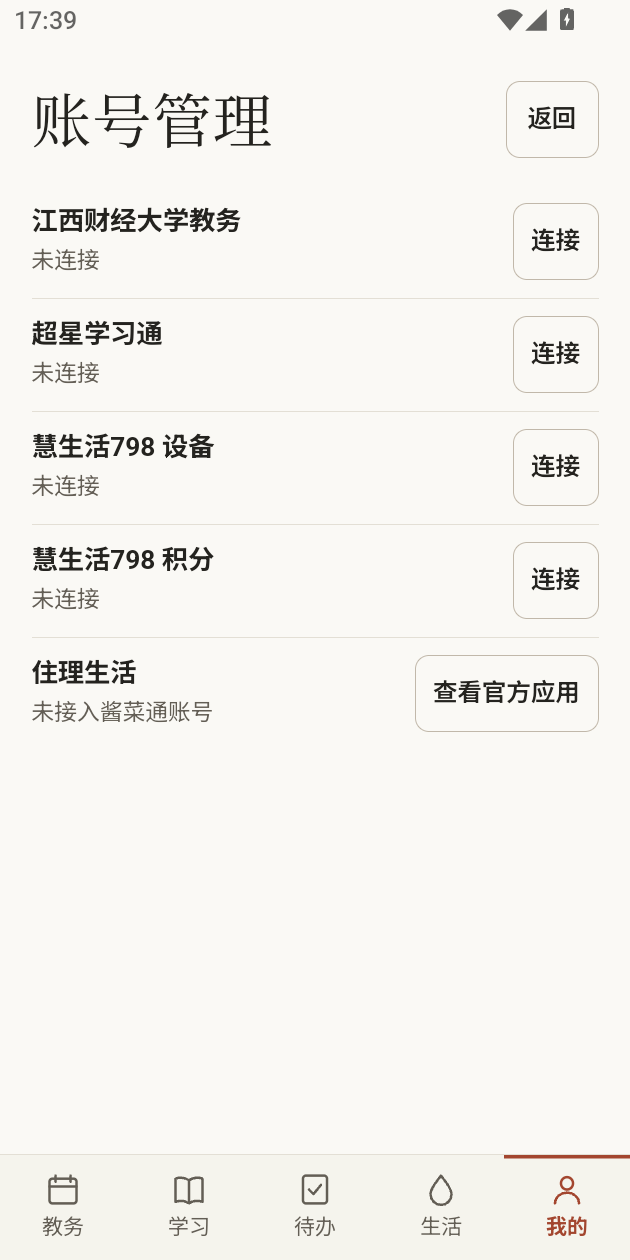
\includegraphics[width=.46\linewidth,trim=0bp 466bp 0bp 34bp,clip]{after-accounts.png} \\
\small （a）生活入口 & \small （b）统一账号管理
\end{tabular}
\caption{生活入口与“我的”账号中心的实际界面}\label{fig:run-other}
\end{figure}

\subsection{典型操作流程}
\textbf{教务查询}\quad 首次从账号中心发起校方登录，然后在教务页选择学期和周次。应用按账号和学期读取本机结果，确认可访问时再读取校方个人课表。课程块可查看详细地点及周次。已验证 261、252 学期的真实课表读取，当前版本重新启动后仍可回读已保存的课表。

\textbf{学习任务}\quad 有效会话下进入学习页，按当前教学班读取或刷新。作业、考试和活动经解析归并，用户从类型与状态筛选切换至按课程查看，再决定是否打开任务链接。实际扫描及教学班分组已通过真实课程检验，窄屏上的筛选和分组另用本地合成任务复核。

\textbf{本地待办}\quad 输入一项任务并添加，打开详情编辑备注，随后勾选完成并从相应筛选项检查结果。用户可取消完成，也可二次确认删除。模拟器中的操作覆盖新增、编辑、筛选、勾选和删除。重新加载后，已保存的记录可以恢复。

\textbf{饮水查询}\quad 设备账号本人验证成功后，返回生活页查看余额、收藏设备与消费账单。真实账户实验核对了这三项结果，重新启动应用后也可再次查询。新版页面复核覆盖了饮水入口和账号界面。

\subsection{实验结果与分析}
表\ref{tab:validation}汇总了主要实验及其运行结果。课表、成绩、学习任务和用水账户的真实查询检验了应用与各服务的数据交互。界面操作和合成输入分别用于验证日常操作及边界行为。考试开放批次返回了空报表，住理生活原生功能也尚未取得真实业务结果，两者的验证范围在表中单列说明。

\begin{table}[htbp]
\centering\small
\caption{主要功能的测试内容与运行结果}\label{tab:validation}
\begin{tabularx}{\linewidth}{@{}>{\raggedright\arraybackslash}p{24mm}>{\raggedright\arraybackslash}p{43mm}Y@{}}
\toprule
功能模块 & 测试内容 & 运行结果 \\
\midrule
教务 & 真实课表读取、静默刷新、成绩切换与缓存回读 & 课表可读取并更新，四个成绩学期可切换。考试开放批次仅返回真实空报表，非空记录解析待核查。 \\
学习通 & 实际课程扫描、课程分组、隐藏课程复查及筛选 & 实际读取课程及任务，隐藏项可参与复查。筛选和自动恢复规则另经合成检查，长期恢复仍待观测。 \\
本地待办 & 新增、编辑、勾选、筛选、删除及重启 & 模拟器操作通过，已保存记录可恢复。带可见软键盘的遮挡情况仍待设备复核。 \\
慧生活798 & 设备账号登录及重启后查询 & 实际读取余额、收藏设备和账单。积分登录、兑换及设备启停待验证。 \\
住理生活 & 官方应用入口、设备选择页及连接状态 & 可打开官方入口，已观察设备选择页。本机状态处理经合成检查，原生查询与控制仍待接入。 \\
导航与账号 & 安装启动、服务入口、主题切换 & 五项导航和账号入口可用，深浅主题可切换。界面检查覆盖当前版本，线上查询结论来自前述业务实验。 \\
\bottomrule
\end{tabularx}
\end{table}

\FloatBarrier
\Needspace{15\baselineskip}
\section{总结与反思}

\subsection{阶段成果}
项目将分散的教务、教学与校园生活入口放入同一应用。课表作为首页提供按学期及周次查询，学习页把跨教学班任务集中展示。本地待办构成可在离线条件下独立使用的场景，统一账号中心承担外部会话的操作入口。已核对的动态数据主要来自校方课表和有效成绩、学习通任务及798用水账户。现场可从离线课表和本地待办开始演示，具备有效会话时再进入在线查询。

\subsection{技术难点与解决思路}
教务登录循环使我认识到，用户授权和会话核验虽访问同一个门户，却不能共用界面恢复的触发条件。单测能够验证失效状态是否回写，只有覆盖安装后的实际启动和返回操作才能观察窗口是否再次弹出。798 的经历则说明，网络链路的验收应从真实服务结果倒推。申请短信、提交验证码、读取账户数据是三项不同的验证，某一环成功不应代替下一环的证据。将这些环节分开检查后，问题复现和修复验证可以使用相同的操作条件。

\subsection{AI 辅助开发与个人贡献}
我从江财学生换教室、查作业、记录个人安排和使用校园服务的场景出发，确定了五个模块的分工及统一账号入口。我确定课表优先回读、失效后主动重连的处理目标，也要求课程活跃度依据作业和通知判断，隐藏课程仍有机会在后续检查中恢复。开发中使用 Codex 辅助整理需求、阅读参考源码、编写及修改代码、排查故障、运行构建和定向测试，也辅助整理本报告及图表。我依据真实使用过程确认教务有效成绩的查询条件，亲自在授权页面完成必要登录，在真机复查798问题并反馈，发现单项调整仍无法登录后，锁定问题完成修复，并在新版上本人完成验证码验证，确认设备账号恢复。在校方返回空报表时，先回到真实页面核实查询条件；设备端持续登录失败时，提供可用参考包，把问题转为对照两个实际客户端。界面调整后则核对原事件绑定和前后截图。通过这些复核，代码修改可以对应到具体操作，假设、合成结果和真实服务结果也能在报告中分别说明。

\subsection{不足与后续计划}
目前需要优先补齐现场可复验的空白。教务应在校方开放真实非空考试安排后核对日期、地点和考试批次。学习通应继续观察真实新任务发布后的恢复行为，保留分项未读全时的提示。积分及设备启停涉及真实账户或扣费，验证须由用户本人发起。下一步继续开发洗浴原生能力，完善功能实现。

\Needspace{8\baselineskip}
\begingroup
\small
\linespread{1.12}\selectfont
\setlength{\bibitemsep}{2pt}
\printbibliography[heading=bibliography,title={参考资料}]
\endgroup
\end{document}
